\todo{Provide Verilog idioms for each of the sequential circuits}

\todo{The build up of SR latch is interesting from here.}
\url{https://www.youtube.com/watch?v=BYN8Zmk6HJY}

\todo{JK latch and T ff are not that interesting}

\todo{Metastability must be introduced}

\section{Objectives}
\begin{enumerate}
  \item Understand timing diagrams, gate delays and critical path
  \item Design Hazard-free two level circuits
  \item Building blocks of sequential circuits
  \item Analyze a sequential circuit and derive a state-table and a state-graph
  \item Derive a state graph or state table from a word description of the problem
  \item Understanding the structure of an FPGA
\end{enumerate}

\section{Why do we need sequential circuits?}

\begin{example}
  Think about this problem: Design an occupancy counter that depends on a
  sensor $S$ at the class door. The sensor is triggered every time a person passes
  through the door. The counter can be reset to zero with a reset button. Assume
  we only need up to two bit counter $C_1C_0$. Draw a truth table for this
  circuit. Do you have requisite knowledge for designing this circuit? Can this
  circuit be designed without a memory element?
\end{example}
\vspace{10em}


\section{Timing diagrams and propagation delays}

\begin{example}[Timing diagram]
  Draw a timing diagram for an ideal NAND gate.
\end{example}
\vspace{20em}

\subsection{Delays}
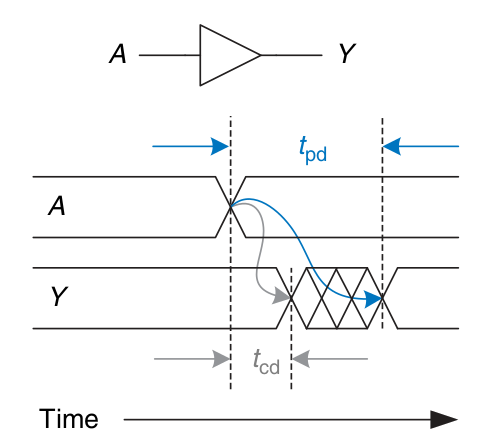
\includegraphics[width=0.5\linewidth]{fig/fig2.67-delays-tpd-tcd.png}
\begin{definition}[Propagation delay ($t_{pd}$)]
\end{definition}
\vspace{5em}

\begin{definition}[Contamination delay ($t_{cd}$)]
\end{definition}
\vspace{5em}

\subsection{Paths}
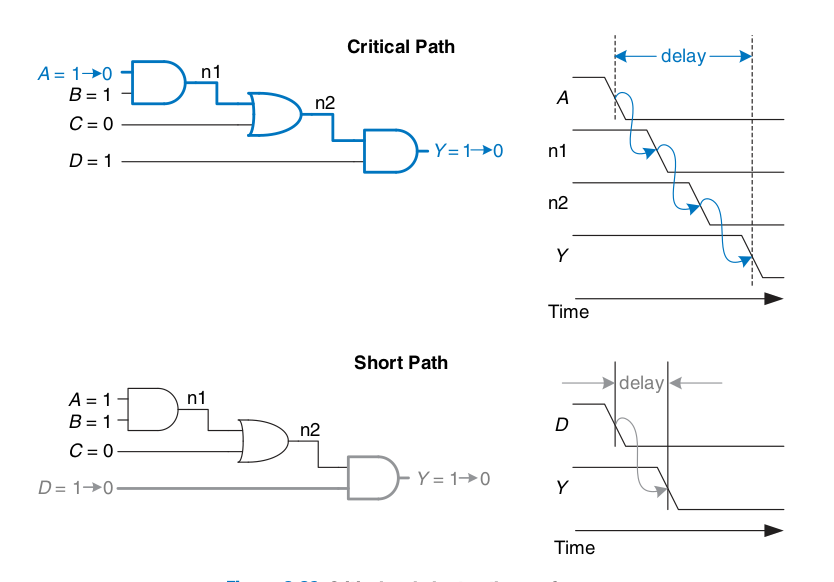
\includegraphics[width=0.8\linewidth]{fig/fig2.68-short-path-and-critical-path.png}
\begin{example}
  Find the propagation delay of the circuit above given that propagation delay
  of each gate is $100 ps$  add contamination delay of $60ps$.
\end{example}
\vspace{10em}

\section{Glitches or Hazards}
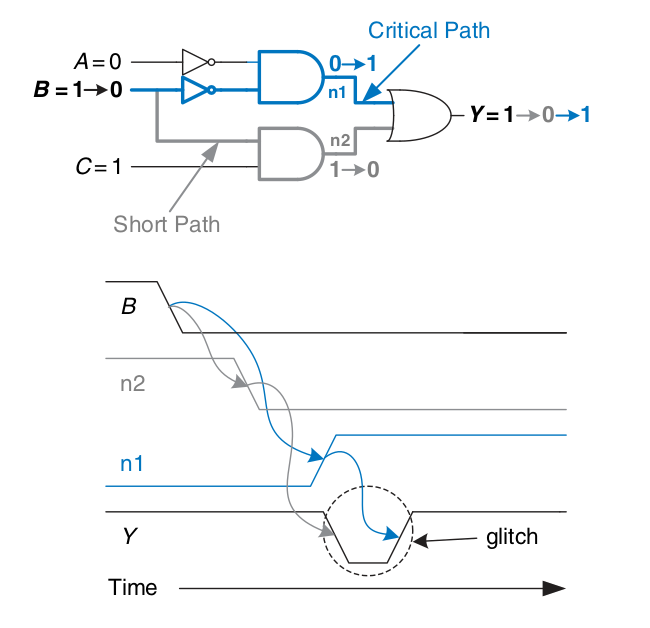
\includegraphics[width=0.6\linewidth]{fig/fig2.76-timing-of-a-glitch.png}
\begin{definition}[Glitch or Hazard]

\end{definition}
\vspace{5em}

\begin{example}
  Design a circuit that fixes the glitch in the above circuit (also known as
  glitch-free or hazard-free circuit).
\end{example}
\vspace{10em}


\section{How to create memory element from circuits}

Two types of memory
\begin{enumerate}
  \item Volatile memory. For example, RAM, CPU registers.
  \item Non-volatile memory. For example, SSD, Flash drives. (Not covered in this course)
    \begin{enumerate}
    \item Memories that require periodic refreshing. For example, DRAM: Dynamics Random Access memory (Not covered in this course)\\
      \includegraphics[width=0.6\linewidth]{./fig/DRAM-cell.png}~\footnote{Image
        source: \url{allaboutcircuits.com/technical-articles/introduction-to-dram-dynamic-random-access-memory/}}
    \item Memories that are always refreshing. For example, SRAM: Static Random
      Access memory~\cite[Appendix~B.64]{stephen2022fundamentals}\\
      \includegraphics[width=0.4\linewidth]{./fig/SRAM-cell.png}
    \end{enumerate}
\end{enumerate}

\section{Latches and Flip-Flops \cite[Sec~3.2]{harris2022digital}}

\begin{example}[Ring oscillator ] \cite[Sec~3.31]{harris2022digital}
  How many stable states does the following circuit have?\\
  \includegraphics[width=0.6\linewidth]{./fig/ring-oscillator.pdf} 
\end{example}
\vspace{10em}

\begin{definition}[Astable circuits]
\end{definition}
\vspace{5em}


\begin{example}
  Analyze the timing diagram of the following circuit.\\
  \includegraphics[width=0.4\linewidth]{./fig/simple-memory-element.png}
\end{example}
\vspace{10em}

\begin{definition}[Bistable circuits]
\end{definition}
\vspace{5em}

\begin{definition}[Characteristic or state table]
  Draw the characteristic or state table of the above circuit. 
\end{definition}
\vspace{10em}



\subsection{SR (Set-Reset) latch \cite[Sec~3.2.1]{harris2022digital}}

\begin{definition}[SR latch]
  The following circuit is called the SR latch. \\
  \includegraphics[width=0.3\linewidth]{./fig/fig3.3-SR-latch.png} \\
  \begin{enumerate}
    \item How many stable states does this circuit have?
    \item Draw its characteristic or state table.
    \item Draw SR latch symbol
  \end{enumerate}
\end{definition}
\vspace{20em}


\begin{prob}[SR latch using NAND gates]
Draw the characteristic or state table for the following circuit\\
  \includegraphics[width=0.3\linewidth]{./fig/fig3.65-SR-NAND-latch.png} \\
\end{prob}

\subsection{Gated SR latch \cite[Sec~5.2]{stephen2022fundamentals}}

\begin{definition}[Gated SR latch]
  The following circuit is called the Gated SR latch. \\
  \includegraphics[width=0.6\linewidth]{./fig/gated-SR-latch.png} \\
  \begin{enumerate}
  \item Draw its characteristic table.
  \item Draw the Gated SR latch symbol
  \end{enumerate}
\end{definition}
\vspace{20em}

\subsection{D (Data) latch \cite[Sec~3.2.2]{harris2022digital}}

\begin{definition}[D latch]
  The following circuit is called the D latch. \\
  \includegraphics[width=0.6\linewidth]{./fig/fig3.7-D-latch.png} \\
  \begin{enumerate}
  \item Draw its characteristic table.
  \item Draw the D latch symbol
  \end{enumerate}
\end{definition}
\vspace{20em}

\subsection{D flip-flop \cite[Sec~3.2.2]{harris2022digital}}

\begin{definition}[D flip-flop]
  The following circuit is called the D flip-flop. \\
  \includegraphics[width=0.6\linewidth]{./fig/fig3.8-D-flip-flop.png} \\
  \begin{enumerate}
  \item Draw its timing  diagram
  \item Draw its characteristic table.
  \item Draw the D flip-flop symbol
  \end{enumerate}
\end{definition}
\vspace{20em}

\begin{remark}
  What is the difference between a latch and a flip-flop?
\end{remark}
\vspace{5em}

\begin{example}
  Add a \emph{RESET} signal to the D flip-flop that resets the state of flip-flop to 0.
\end{example}
\vspace{20em}

\begin{example}
  The toggle (T) flip-flop has one input, CLK, and one output, Q. On
  each rising edge of CLK, Q toggles to the complement of its previous value. Draw
  a schematic for a T flip-flop using a D flip-flop and an inverter.
\end{example}
\vspace{20em}

\begin{prob}
  A JK flip-flop receives a clock and two inputs, J and K. On the rising
  edge of the clock, it updates the output, Q. If J and K are both 0, Q retains its old
  value. If only J is 1, Q becomes 1. If only K is 1, Q becomes 0. If both J and K are 1,
  Q becomes the opposite of its present state.
  \begin{enumerate}
  \item Construct a JK flip-flop using a D flip-flop and some combinational logic.
  \item Construct a D flip-flop using a JK flip-flop and some combinational logic.
  \item Construct a T flip-flop (see Exercise 3.9) using a JK flip-flop.
  \end{enumerate}
\end{prob}


\section{Finite State Machines~\cite[Sec~3.4]{harris2022digital}}\footnote{These
  notes will not fit on your note sheet.}

\begin{example}
  Design an occupancy counter that depends on a
  sensor $S$ at the class door. The sensor is triggered every time a person passes
  through the door. Assume that the counter starts at zero. Assume
  we only need up to two bit counter $C_1C_0$. Draw a state table for this
  circuit.
\end{example}

\begin{prob}
  A divide-by-N counter has one output and no inputs. The output Y is HIGH for
  one clock cycle out of every N. In other words, the output divides the frequency
  of the clock by N. The waveform for a divide-by-3 counter is shown here:\\
  \includegraphics[width=0.8\linewidth]{./fig/fig.38a-divide-by-3-counter.png}\\
  Sketch circuit designs for such a counter
\end{prob}

\begin{prob}
  Design a 3-bit counter which counts in the sequence:
  001, 011, 010, 110, 111, 100, (repeat) 001, ...
\end{prob}

\begin{example}
  Design an odd-even counter for an single bit input. The output of this circuit
  should be 1 if the number of 1s to the input have been odd so far and 0
  otherwise.
\end{example}

\begin{example}[Sequence detectors]
  A sequential circuit has one input and one output. The output becomes 1 and
  remain 1 thereafter when at least two 0's and at least two 1's have occurred
  as inputs regardless of the order of 
\end{example}

\begin{example}
  Consider the problem of inventing a controller for a traffic light at a busy
  intersection on campus. There are two traffic
  sensors, $T_A$ and $T_B$ , on Academic Ave. and Bravado Blvd., respectively.
  Each sensor indicates TRUE if students are present and FALSE if the
  street is empty. There are two traffic lights, $L_A$ and $L_B$, to control
  traffic. Each light receives digital inputs specifying whether it should be
  green, yellow, or red.
  When the system is reset, the lights are green on Academic Ave. and red on Bravado Blvd.
  As long as traffic is present on Academic Ave., the lights do not change. When there
  is no longer traffic on Academic Ave., the light on Academic Ave.
  becomes yellow for 5 seconds before it turns red and Bravado Blvd.’s light
  turns green. Similarly, the Bravado Blvd. light remains green as long as
  traffic is present on the boulevard, then turns yellow and eventually red.
  \\
  \includegraphics[width=0.5\linewidth]{./fig/fig3.23-campus-map.png}
  \includegraphics[width=0.5\linewidth]{./fig/fig3.24-traffic-light-controller.png}
  \begin{enumerate}
  \item Draw a state transition diagram
  \item Draw a state table 
  \item Assign binary encodings to each of the states
  \item Redraw the state table with binary encodings. Design a minimal SOP
    boolean expression.
  \item Assign binary encodings to each of the output and redraw the output
    table. Design a minimal SOP boolean expression for the outputs.
  \end{enumerate}
\end{example}


\begin{prob}
  Design a circuit for a 2x2 pixel resolution pong game, where the ball can only
  occupy 4 possible pixels and a single paddle occupies another 2 pixels. The
  ball bounces of the paddle when the paddle is in the correct row. To keep it
  interesting, the ball takes a different path from the source path. Track the
  score with a single bit counter.
\end{prob}
